\documentclass[11pt,a4paper]{article}
\usepackage[margin=2.2cm]{geometry}
\usepackage[T1]{fontenc}
\usepackage{lmodern}
\usepackage{booktabs}
\usepackage{tabularx}
\usepackage{xcolor}
\usepackage{textcomp}
\usepackage{listings}
\usepackage{tikz}
\usetikzlibrary{arrows.meta,positioning,calc,shapes.geometric}
\usepackage{pgfplots}
\pgfplotsset{compat=1.17}
\usepackage{caption}
\usepackage{float}
\usepackage{enumitem}
\usepackage[hidelinks]{hyperref}

\definecolor{codebg}{RGB}{246,247,249}
\definecolor{llm}{RGB}{219,234,254}
\definecolor{tool}{RGB}{220,252,231}
\definecolor{io}{RGB}{243,244,246}
\definecolor{passc}{RGB}{34,139,84}
\definecolor{failc}{RGB}{200,60,60}

\lstset{
  basicstyle=\ttfamily\footnotesize, backgroundcolor=\color{codebg},
  frame=single, rulecolor=\color{black!15}, breaklines=true, columns=fullflexible,
  keepspaces=true, showstringspaces=false, upquote=true, aboveskip=6pt, belowskip=6pt,
  keywordstyle=\color{blue!60!black}\bfseries, commentstyle=\color{black!55}
}
\lstdefinestyle{prompt}{language={}, basicstyle=\ttfamily\scriptsize}
\setlist{itemsep=2pt, topsep=4pt}
\emergencystretch=3em

\title{\textbf{Agentic AI Pipeline for Coverage-Directed Unit Testing}\\[4pt]
\large CSE731: Software Testing --- Mid-term Project, Term I (2026--27)}
\author{Krish Patel (IMT2023134) \quad Yash Gupta (IMT2023125)}
\date{October 2026}

\begin{document}
\maketitle

\begin{abstract}
We built a pipeline of three agents, written in plain Java, that generates a unit of code, generates JUnit~5 unit tests that must reach a user-specified coverage criterion, and executes those tests to give a verdict. The test case generator follows option~(1) of the problem statement: a coverage criterion (statement or branch coverage, measured with JaCoCo). The test case executor's measured coverage gaps are fed back to the test case generator for up to three rounds. On the first 12 problems of HumanEval-X (Java), with a 100\% branch-coverage target, 8 of 12 tasks reached the goal with all tests passing. Three of the remaining four contain branches that no valid input can reach.
\end{abstract}

\noindent\textbf{Code repository:} \url{https://github.com/kodercrish/Software-Testing}

\section{Pipeline}

\subsection{Overview}
The pipeline consists of three agents, connected by an ordinary Java loop (\texttt{Pipeline.java}). As the project rules require, it uses no agent framework, no RAG and no chain-of-thought: each LLM agent is a single HTTP request to an OpenAI-compatible chat API (OpenRouter).

\begin{figure}[H]
\centering
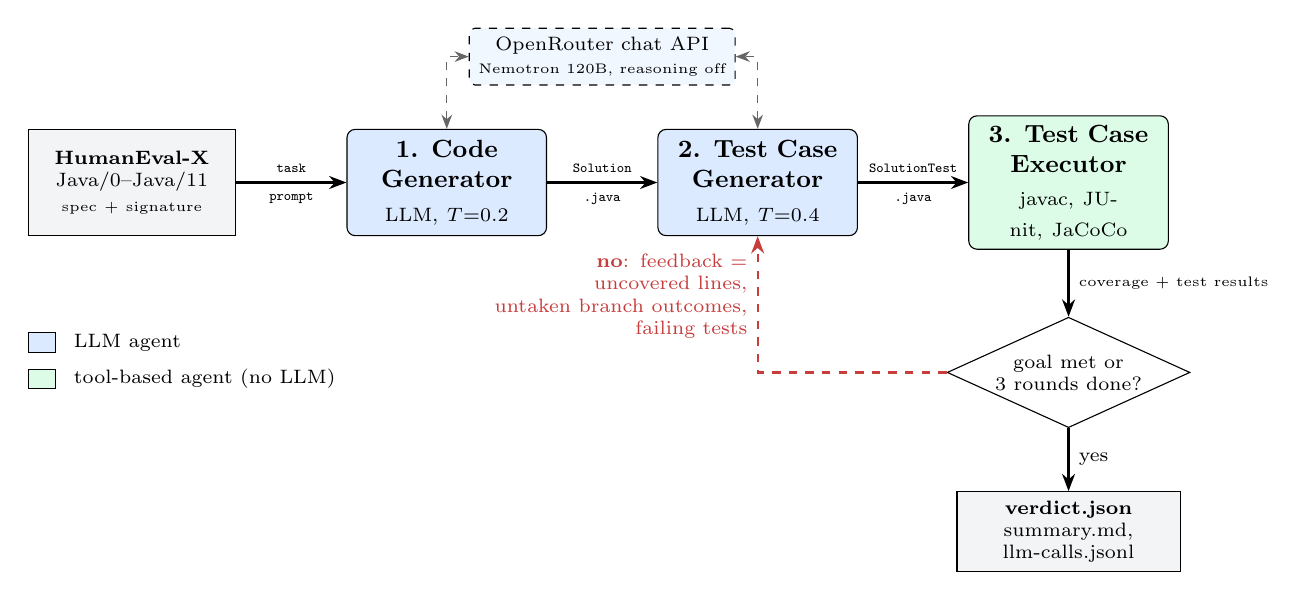
\begin{tikzpicture}[
  box/.style={draw, rounded corners=3pt, align=center, minimum height=1.35cm, text width=2.3cm, font=\small},
  data/.style={draw, align=center, fill=io, font=\scriptsize},
  arr/.style={-{Stealth[length=2.2mm]}, thick},
  lbl/.style={font=\tiny\ttfamily, align=center}]
  % main row
  \node[data, text width=2.4cm, minimum height=1.35cm] (ds) {\textbf{HumanEval-X}\\Java/0--Java/11\\[1pt]{\tiny spec + signature}};
  \node[box, fill=llm, right=1.4cm of ds] (cg) {\textbf{1. Code}\\\textbf{Generator}\\[1pt]{\scriptsize LLM, $T{=}0.2$}};
  \node[box, fill=llm, right=1.4cm of cg] (tg) {\textbf{2. Test Case}\\\textbf{Generator}\\[1pt]{\scriptsize LLM, $T{=}0.4$}};
  \node[box, fill=tool, right=1.4cm of tg] (ex) {\textbf{3. Test Case}\\\textbf{Executor}\\[1pt]{\scriptsize javac, JUnit, JaCoCo}};
  % LLM API shared by agents 1 and 2
  \node[draw, dashed, rounded corners=2pt, fill=llm!40, font=\scriptsize, align=center, above=0.55cm of $(cg.north)!0.5!(tg.north)$] (api)
       {OpenRouter chat API\\{\tiny Nemotron 120B, reasoning off}};
  % decision and outputs
  \node[diamond, draw, aspect=2.2, inner sep=1pt, font=\scriptsize, align=center, below=0.85cm of ex] (dec) {goal met or\\3 rounds done?};
  \node[data, text width=2.6cm, below=0.8cm of dec] (out) {\textbf{verdict.json}\\summary.md, llm-calls.jsonl};
  % flow
  \draw[arr] (ds) -- node[lbl, above]{task} node[lbl, below]{prompt} (cg);
  \draw[arr] (cg) -- node[lbl, above]{Solution} node[lbl, below]{.java} (tg);
  \draw[arr] (tg) -- node[lbl, above]{SolutionTest} node[lbl, below]{.java} (ex);
  \draw[arr] (ex) -- node[lbl, right, font=\tiny]{coverage + test results} (dec);
  \draw[arr] (dec) -- node[font=\scriptsize, right]{yes} (out);
  \draw[arr, dashed, color=failc] (dec.west) -| node[pos=0.78, left, font=\scriptsize, align=right, text width=3.6cm, color=failc]
       {\textbf{no}: feedback =\\uncovered lines,\\untaken branch outcomes,\\failing tests} (tg.south);
  \draw[{Stealth[length=1.8mm]}-{Stealth[length=1.8mm]}, dashed, color=black!60] (cg.north) |- (api.west);
  \draw[{Stealth[length=1.8mm]}-{Stealth[length=1.8mm]}, dashed, color=black!60] (tg.north) |- (api.east);
  % legend
  \node[draw, fill=llm, minimum width=0.35cm, minimum height=0.25cm, below=1.35cm of ds.south west, anchor=west] (l1) {};
  \node[font=\scriptsize, right=0.1cm of l1] (l1t) {LLM agent};
  \node[draw, fill=tool, minimum width=0.35cm, minimum height=0.25cm, below=0.2cm of l1] (l2) {};
  \node[font=\scriptsize, right=0.1cm of l2] {tool-based agent (no LLM)};
\end{tikzpicture}
\caption{The agentic pipeline for one task. Agents 1 and 2 call the LLM; agent 3 runs real tools. If the coverage goal is not met, the executor's findings go back to the test case generator (red, dashed).}
\label{fig:pipeline}
\end{figure}

\subsection{Dataset}
We use the Java split of \textbf{HumanEval-X} (164 problems), and run the pipeline on the first 12 (\texttt{Java/0}--\texttt{Java/11}). Each problem's \texttt{prompt} contains the imports, \texttt{class Solution}, a Javadoc specification with examples, and the method signature. Only this prompt is given to the agents.

\subsection{Testing goal: user-specified coverage criterion}
The user sets the criterion and the target in \texttt{config.properties}:
\begin{itemize}
  \item \texttt{STATEMENT}: every executable statement is run by some test (JaCoCo \emph{line} counter);
  \item \texttt{BRANCH}: every decision (\texttt{if}, loop condition, \texttt{\&\&}, \texttt{||}, \texttt{?:}) evaluates to both \emph{true} and \emph{false} (JaCoCo \emph{branch} counter). This corresponds to edge coverage of the method's control-flow graph.
\end{itemize}
For the experiments we used \texttt{BRANCH} with a target of 100\%.

\subsection{The three agents}
\begin{description}
  \item[1. Code Generator (LLM).] Receives the task prompt and returns one compilation unit, \texttt{Solution.java}. The Java code block is extracted from the reply.
  \item[2. Test Case Generator (LLM).] Receives the specification and the generated code \emph{with line numbers}, and returns \texttt{SolutionTest.java} (JUnit~5). It is told to derive expected values from the \emph{specification}, not from the implementation, so that tests can reveal bugs. In a feedback round it also receives the executor's report and the current tests, and returns an improved test class.
  \item[3. Test Case Executor (no LLM).] Compiles and runs the tests in a separate JVM, measures coverage and decides the verdict (Figure~\ref{fig:executor}). Because the verdict comes from real execution, it is objective and reproducible.
\end{description}

\begin{figure}[H]
\centering
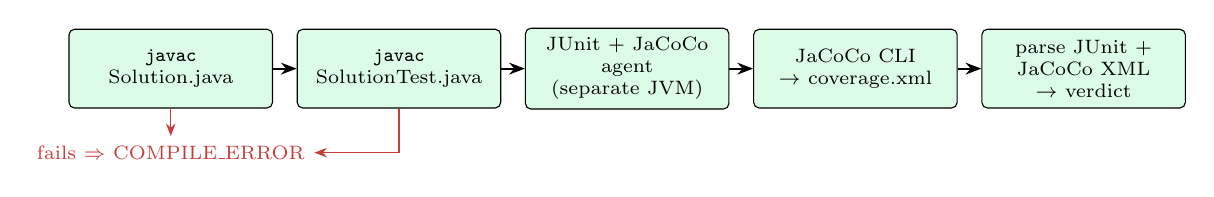
\begin{tikzpicture}[
  node distance=0.3cm,
  st/.style={draw, rounded corners=2pt, fill=tool, font=\scriptsize, align=center, minimum height=1.0cm, text width=2.35cm},
  arr/.style={-{Stealth[length=2mm]}, thick}]
  \node[st] (a) {\texttt{javac}\\Solution.java};
  \node[st, right=of a] (b) {\texttt{javac}\\SolutionTest.java};
  \node[st, right=of b] (c) {JUnit + JaCoCo\\agent\\(separate JVM)};
  \node[st, right=of c] (d) {JaCoCo CLI\\$\rightarrow$ coverage.xml};
  \node[st, right=of d] (e) {parse JUnit +\\JaCoCo XML\\$\rightarrow$ verdict};
  \draw[arr] (a) -- (b); \draw[arr] (b) -- (c); \draw[arr] (c) -- (d); \draw[arr] (d) -- (e);
  \node[font=\scriptsize, color=failc, below=0.35cm of a] (ce) {fails $\Rightarrow$ COMPILE\_ERROR};
  \draw[-{Stealth[length=1.6mm]}, color=failc] (a) -- (ce);
  \draw[-{Stealth[length=1.6mm]}, color=failc] (b.south) |- (ce.east);
\end{tikzpicture}
\caption{Steps of the Test Case Executor. Every process has a 30\,s timeout.}
\label{fig:executor}
\end{figure}

\noindent The verdict is decided by four rules, checked in order:
\begin{center}
\begin{tabular}{@{}ll@{}}
\toprule
Condition & Verdict \\
\midrule
code or tests do not compile & \texttt{COMPILE\_ERROR} \\
no test ran, or any test failed & \texttt{TESTS\_FAILED} \\
all tests pass, coverage $<$ target & \texttt{COVERAGE\_NOT\_MET} \\
all tests pass, coverage $\geq$ target & \texttt{PASS} \\
\bottomrule
\end{tabular}
\end{center}

\subsection{Feedback loop}
If the goal is not met, the executor's results are turned into a plain-text report and sent back to the test case generator. The report lists the uncovered lines with their source text, the decisions with untaken outcomes, failing tests with their messages, and compile errors. The loop stops when the goal is met, when the generated code itself does not compile, or after \texttt{maxTestIterations}~=~3 rounds. The verdict of the last round is reported.

\section{Prompts and Settings}

\begin{table}[H]
\centering
\begin{tabular}{@{}lll@{}}
\toprule
Setting & Code Generator & Test Case Generator \\
\midrule
Model & \multicolumn{2}{l}{\texttt{nvidia/nemotron-3-super-120b-a12b:free} via OpenRouter} \\
Reasoning (``thinking'') & disabled & disabled \\
temperature & 0.2 & 0.4 \\
top\_p & 0.95 & 0.95 \\
max\_tokens & 2048 & 4096 \\
seed & 42 & 42 \\
Other & --- & criterion = BRANCH, target = 100\%, max.\ 3 rounds \\
\bottomrule
\end{tabular}
\caption{Model and sampling settings.}
\end{table}

\begin{itemize}
  \item The code generator uses a low temperature to get the most likely correct solution.
  \item The test generator uses a slightly higher temperature, so that it tries more varied inputs when it must reach uncovered branches.
  \item The model's built-in reasoning mode is switched off in every request (\texttt{"reasoning": \{"enabled": false\}}), so it answers directly without a hidden chain of thought.
  \item The free model is sometimes rate-limited, so the client retries a failed request after 20\,s, up to 6 times.
\end{itemize}

\noindent The prompts are plain-text templates. Placeholders \texttt{\{\{...\}\}} are filled in at run time, and every request and response is logged in \texttt{llm-calls.jsonl}.

\subsubsection*{Code Generator, system prompt}
\begin{lstlisting}[style=prompt]
You are a code generator agent in an automated unit-testing pipeline.
You write correct, compilable Java 21 code that implements a specification.

Rules:
- Output exactly one Java code block (```java ... ```) and nothing else.
- The code block must be a complete compilation unit: the given imports and the class `Solution`
  containing the requested method with the exact given signature. Helper methods are allowed inside `Solution`.
- Do not add a package declaration, a main method, or any other top-level class.
- Use only the Java standard library.
\end{lstlisting}
\subsubsection*{Code Generator, user prompt}
\begin{lstlisting}[style=prompt]
Implement the method described by the Javadoc below. Keep the class name, method name, parameter types and return type exactly as given.

```java
{{prompt}}
```
\end{lstlisting}
\subsubsection*{Test Case Generator, system prompt}
\begin{lstlisting}[style=prompt]
You are a test case generator agent in an automated unit-testing pipeline.
You write JUnit 5 unit tests for a single Java method.

Testing goal: {{criterion}}. Target: {{target}}% as measured by JaCoCo.

Rules:
- Output exactly one Java code block (```java ... ```) and nothing else.
- The code block is a complete compilation unit containing the class `SolutionTest` (no package declaration).
- Import org.junit.jupiter.api.Test and static org.junit.jupiter.api.Assertions.*, plus any java.util classes you use.
- Create the object under test with `new Solution()`.
- Choose inputs so that the testing goal is reached: every statement / every decision outcome of the
  given implementation must be exercised by at least one test.
- Derive every expected value from the SPECIFICATION (the Javadoc and its examples), not from the implementation,
  so that a test fails if the implementation is wrong.
- One scenario per @Test method, with a descriptive method name. Use assertEquals / assertTrue / assertFalse;
  for doubles use assertEquals(expected, actual, 1e-6).
- Do not use mocking libraries, parameterized tests, reflection, randomness, or file / network I/O.
\end{lstlisting}
\subsubsection*{Test Case Generator, user prompt}
\begin{lstlisting}[style=prompt]
Specification of the method under test:

```java
{{prompt}}
```

Implementation under test (Solution.java, with line numbers):

```
{{numberedCode}}
```

Write the JUnit 5 class `SolutionTest`.
\end{lstlisting}
\subsubsection*{Test Case Generator, feedback prompt (appended to the user prompt in rounds 2 and 3)}
\begin{lstlisting}[style=prompt]
The Test Executor ran your tests. Results:

{{feedback}}

Current SolutionTest.java:

```java
{{tests}}
```

Return the complete improved `SolutionTest` class in one Java code block.
- Add tests that exercise the uncovered lines / branch outcomes listed above.
- If a failing test's expected value contradicts the specification, fix that test. If it agrees with the
  specification, keep it unchanged: it may have found a bug in the implementation.
- Keep all existing passing tests.
\end{lstlisting}

\section{Formats of Code, Tests and Verdict}
\begin{itemize}
  \item \textbf{Code:} one Java file \texttt{Solution.java} containing \texttt{class Solution} with the required method.
  \item \textbf{Tests:} one JUnit~5 file \texttt{SolutionTest.java} with one scenario per \texttt{@Test} method.
  \item \textbf{Verdict:} \texttt{verdict.json}, written by the test case executor.
\end{itemize}
As a sample we show task \texttt{Java/11} (\texttt{stringXor}), which needed one feedback round.

\subsubsection*{Generated code (\texttt{Solution.java})}
\begin{lstlisting}[language=Java]
import java.util.*;
import java.lang.*;

class Solution {
    /**
    Input are two strings a and b consisting only of 1s and 0s.
    Perform binary XOR on these inputs and return result also as a string.
    >>> stringXor("010", "110")
    "100"
     */
    public String stringXor(String a, String b) {
        StringBuilder result = new StringBuilder();
        int length = Math.max(a.length(), b.length());
        for (int i = 0; i < length; i++) {
            char bitA = i < a.length() ? a.charAt(a.length() - 1 - i) : '0';
            char bitB = i < b.length() ? b.charAt(b.length() - 1 - i) : '0';
            char xorBit = (bitA == bitB) ? '0' : '1';
            result.insert(0, xorBit);
        }
        return result.toString();
    }
}
\end{lstlisting}

\subsubsection*{Generated tests, final round (\texttt{SolutionTest.java})}
\begin{lstlisting}[language=Java]
import org.junit.jupiter.api.Test;
import static org.junit.jupiter.api.Assertions.*;

class SolutionTest {
    @Test
    void testEqualLengthBothZeros() {
        Solution sol = new Solution();
        assertEquals("000", sol.stringXor("000", "000"));
    }

    @Test
    void testEqualLengthBothOnes() {
        Solution sol = new Solution();
        assertEquals("000", sol.stringXor("111", "111"));
    }

    @Test
    void testEqualLengthMixed() {
        Solution sol = new Solution();
        assertEquals("110", sol.stringXor("101", "011"));
    }

    @Test
    void testFirstLonger() {
        Solution sol = new Solution();
        assertEquals("1001", sol.stringXor("1100", "101"));
    }

    @Test
    void testSecondLonger() {
        Solution sol = new Solution();
        assertEquals("1001", sol.stringXor("101", "1100"));
    }

    @Test
    void testOneEmpty() {
        Solution sol = new Solution();
        assertEquals("101", sol.stringXor("", "101"));
    }

    @Test
    void testBothEmpty() {
        Solution sol = new Solution();
        assertEquals("", sol.stringXor("", ""));
    }

    @Test
    void testSingleCharDifferent() {
        Solution sol = new Solution();
        assertEquals("1", sol.stringXor("0", "1"));
    }

    @Test
    void testSingleCharSame() {
        Solution sol = new Solution();
        assertEquals("0", sol.stringXor("1", "1"));
    }
}
\end{lstlisting}

\subsubsection*{Verdict (\texttt{verdict.json})}
\begin{lstlisting}[language={}]
{
  "taskId": "Java/11",
  "status": "PASS",
  "testsTotal": 9,
  "testsPassed": 9,
  "criterion": "BRANCH",
  "target": 100.0,
  "statementPct": 100.0,
  "branchPct": 100.0,
  "iterations": 2
}
\end{lstlisting}

\section{Execution Results}
The run on 4 October 2026 used tasks \texttt{Java/0}--\texttt{Java/11}, criterion \texttt{BRANCH}, a 100\% target and at most 3 rounds. All artefacts are in \texttt{runs/20261004-182338/}.

\begin{table}[H]
\centering
\footnotesize
\setlength{\tabcolsep}{4.5pt}
\begin{tabular}{@{}llllrrc@{}}
\toprule
Task & Method & Verdict & Tests passed & Stmt.\,\% & Branch\,\% & Rounds \\
\midrule
Java/0  & hasCloseElements     & \textcolor{failc}{COMPILE\_ERROR}    & 0/0   & 0.0   & 0.0   & 3 \\
Java/1  & separateParenGroups  & \textcolor{failc}{TESTS\_FAILED}     & 13/16 & 100.0 & 83.3  & 3 \\
Java/2  & truncateNumber       & \textcolor{passc}{PASS}              & 4/4   & 100.0 & 100.0 & 1 \\
Java/3  & belowZero            & \textcolor{passc}{PASS}              & 6/6   & 100.0 & 100.0 & 1 \\
Java/4  & meanAbsoluteDeviation& \textcolor{passc}{PASS}              & 7/7   & 100.0 & 100.0 & 1 \\
Java/5  & intersperse          & \textcolor{passc}{PASS}              & 5/5   & 100.0 & 100.0 & 1 \\
Java/6  & parseNestedParens    & \textcolor{failc}{COVERAGE\_NOT\_MET}& 9/9   & 100.0 & 93.8  & 3 \\
Java/7  & filterBySubstring    & \textcolor{passc}{PASS}              & 5/5   & 100.0 & 100.0 & 1 \\
Java/8  & sumProduct           & \textcolor{passc}{PASS}              & 5/5   & 100.0 & 100.0 & 1 \\
Java/9  & rollingMax           & \textcolor{passc}{PASS}              & 8/8   & 100.0 & 100.0 & 1 \\
Java/10 & makePalindrome       & \textcolor{failc}{TESTS\_FAILED}     & 10/11 & 100.0 & 91.7  & 3 \\
Java/11 & stringXor            & \textcolor{passc}{PASS}              & 9/9   & 100.0 & 100.0 & 2 \\
\midrule
\multicolumn{7}{@{}l}{\textbf{Coverage goal reached with all tests passing: 8/12 tasks}} \\
\bottomrule
\end{tabular}
\caption{Final verdict per task (last round).}
\label{tab:results}
\end{table}

\begin{figure}[H]
\centering
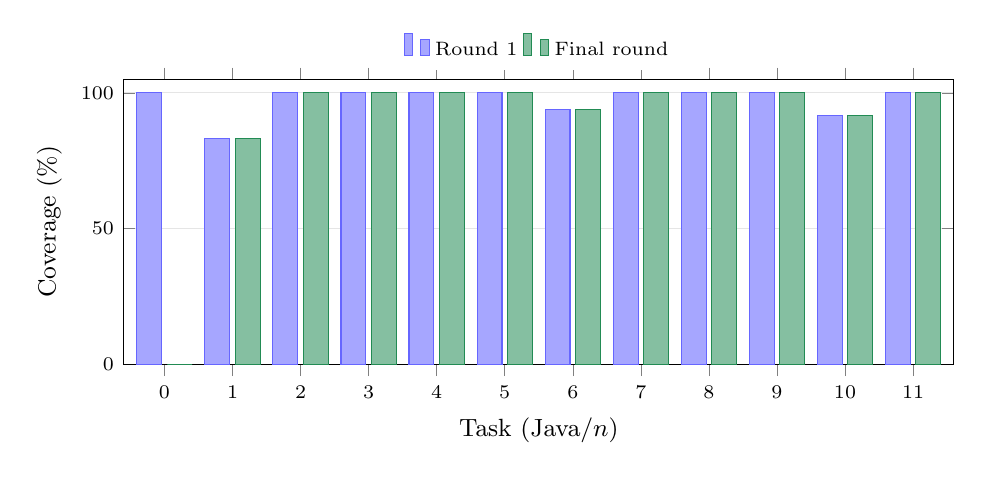
\begin{tikzpicture}
\begin{axis}[
  width=\textwidth, height=5.2cm, ybar, bar width=9pt,
  ymin=0, ymax=105, ylabel={Coverage (\%)},
  xmin=-0.6, xmax=11.6, xtick={0,...,11},
  xlabel={Task (Java/$n$)}, xlabel style={font=\small}, ylabel style={font=\small},
  tick label style={font=\scriptsize},
  legend style={at={(0.5,1.03)}, anchor=south, legend columns=-1, font=\scriptsize, draw=none},
  ymajorgrids, grid style={black!10}]
\addplot[fill=blue!35, draw=blue!60] coordinates {(0,100) (1,83.3) (2,100) (3,100) (4,100) (5,100) (6,93.8) (7,100) (8,100) (9,100) (10,91.7) (11,100)};
\addplot[fill=passc!55, draw=passc] coordinates {(0,0) (1,83.3) (2,100) (3,100) (4,100) (5,100) (6,93.8) (7,100) (8,100) (9,100) (10,91.7) (11,100)};
\legend{Round 1, Final round}
\end{axis}
\end{tikzpicture}
\caption{Branch coverage per task in round 1 and in the final round (target 100\%). For Java/0, the final round did not compile.}
\label{fig:coverage}
\end{figure}

\begin{table}[H]
\centering
\small
\begin{tabular}{@{}lccc@{}}
\toprule
Task & Round 1 & Round 2 & Round 3 \\
\midrule
Java/0  & 9/10 pass, 100.0\% & 9/13 pass, 100.0\% & does not compile \\
Java/1  & 8/8 pass, 83.3\%   & 10/12 pass, 83.3\% & 13/16 pass, 83.3\% \\
Java/6  & 7/7 pass, 93.8\%   & 8/8 pass, 93.8\%   & 9/9 pass, 93.8\% \\
Java/10 & 7/7 pass, 91.7\%   & 9/9 pass, 91.7\%   & 10/11 pass, 91.7\% \\
Java/11 & 7/9 pass, 100.0\%  & 9/9 pass, 100.0\%  & --- \\
\bottomrule
\end{tabular}
\caption{Tasks that used the feedback loop: tests passed and branch coverage per round. All other tasks passed in round 1.}
\label{tab:rounds}
\end{table}

\noindent Feedback sent to the test case generator after round 1 of \texttt{Java/11}:
\begin{lstlisting}[style=prompt]
Coverage: statements 9/9 (100.0%), branches 8/8 (100.0%)
Tests: 9 run, 7 passed, 2 failed
  FAILED testFirstLonger(): expected: <1010> but was: <1001>
  FAILED testSecondLonger(): expected: <1010> but was: <1001>
\end{lstlisting}

\subsection{Discussion}
\begin{itemize}
  \item \textbf{Goal reached in 8 of 12 tasks}, 7 of them in the first round. All tasks whose final round compiled reached 100\% statement coverage.
  \item \textbf{The feedback loop repaired wrong tests.} In \texttt{Java/11} two tests expected wrong XOR results (\texttt{1010} instead of \texttt{1001}). After the executor reported the failures, the generator corrected them in round 2.
  \item \textbf{Infeasible branches (\texttt{Java/1}, \texttt{Java/6}, \texttt{Java/10}).} The uncovered branch outcomes cannot be reached by any input that satisfies the specification:
  \begin{itemize}
    \item In \texttt{Java/1} and \texttt{Java/6}, the \emph{false} outcome of \texttt{else if (c == ')')} needs a character that is neither \texttt{(} nor \texttt{)}, but the input contains only parentheses and spaces.
    \item In \texttt{Java/10}, the exit of the \texttt{for} loop is never reached, because a single character is always a palindromic suffix, so the loop always returns early.
  \end{itemize}
  These are infeasible test requirements: 100\% branch coverage is not achievable for these implementations. Trying anyway, the generator invented invalid inputs (e.g.\ unbalanced parentheses) with guessed expected values, which then failed. An LLM cannot tell an infeasible branch from a hard one.
  \item \textbf{Wrong oracles caught by execution.} Some generated expected values contradict the specification. For example, \texttt{Java/0} expects \texttt{true} for threshold~0, although no difference is smaller than~0, and \texttt{Java/10} expects \texttt{makePalindrome("ab")} to be \texttt{"ababa"} instead of \texttt{"aba"}. Such errors are found only because the verdict comes from running the tests, not from LLM judgement.
  \item \textbf{Regression across rounds (\texttt{Java/0}).} Round 1 already reached 100\% coverage with one wrong test. In round 3 the generator produced duplicate test-method names, so the suite no longer compiled. Since the pipeline reports the last round, the verdict is \texttt{COMPILE\_ERROR}. Keeping the best round would be a simple improvement.
\end{itemize}

\section{Contributions}
The work was split into the LLM side of the pipeline and the execution side.

\begin{table}[H]
\centering
\small
\begin{tabularx}{\textwidth}{@{}lX@{}}
\toprule
Member & Contribution \\
\midrule
Yash Gupta (IMT2023125) & \textbf{Part 1: LLM agents and orchestration.} OpenRouter client (\texttt{LlmClient}), Code Generator agent, Test Case Generator agent including the feedback message, prompt templates and sampling settings (\texttt{Prompts}, \texttt{config.properties}), dataset loader (\texttt{HumanEvalX}), and the pipeline loop (\texttt{Pipeline}, \texttt{Main}). \\
\addlinespace
Krish Patel (IMT2023134) & \textbf{Part 2: Test execution, results and report.} Test Case Executor agent (compiling and running tests with JUnit and JaCoCo, verdict), process runner (\texttt{Proc}), JUnit/JaCoCo report parsing (\texttt{Reports}), run logging and results summary (\texttt{RunLogger}), running the experiments on the 12 tasks, and writing this report. \\
\bottomrule
\end{tabularx}
\end{table}

\end{document}
